
\documentclass[10pt]{llncs}

\hyphenation{op-tical net-works semi-conduc-tor}

\pagestyle{empty}

\usepackage{cite}
\usepackage{color}
\usepackage{url}
\usepackage{algpseudocode}
\usepackage{datapie}
\usepackage{textcomp}
\usepackage{algorithmicx}
\usepackage{listings}
\usepackage{makecell}
\lstset{language=C,
  basicstyle=\ttfamily,
  columns=fullflexible,
  keepspaces=true,
  frame=lines}
\usepackage[normalem]{ulem}
\newcommand\TODO[1]{\uline{\textbf{TODO:} #1}}

\lstdefinestyle{code}{
  language=C,
  basicstyle=\ttfamily\scriptsize,
  columns=fullflexible,
  keepspaces=true,
  moredelim=[is][\underbar]{@}{@}
}
%\IEEEoverridecommandlockouts
\begin{document}

\title{DFTinker: Automated Detecting and Fixing Double-fetch Bugs with Transactional Memory}

\author{
Yingqi Luo\inst{1} \and
Pengfei Wang\inst{1} \and
Xu Zhou\inst{1} \and
Kai Lu\inst{1}}

\institute{National University of Defense Technology, Changsha Hunan, P.R.China}

\maketitle


% \IEEEauthorblockN{Yingqi~Luo,
%         Pengfei~Wang,
%         Xu~Zhou,
%         and~Kai~Lu}
% % \IEEEauthorblockA{\\School of Computer\\
% % National University of Defense Technology\\
% %Changsha Hunan, P.R.China\\
% % }
% \thanks{Y. Luo, P. Wang, X. Zhou and K. Lu are with School of Computer, National University of Defense Technology, No.109, Deya Rd., Changsha City, P.R.China.}
% \thanks{Corresponding author is Y. Luo (email: nudtlyq@163.com)}
%}

\begin{abstract}
%\bfseries
%Double-fetch bugs have attracted great attention in recent years. 
The double-fetch bug is a situation where the operating system kernel fetches the supposedly same data twice from the user space, whereas the data is unexpectedly changed by the user thread. It could cause fatal errors such as kernel crashes, information leakage, and privilege escalation. Previous research focuses on the detection of double-fetch bugs, however, the fix of such bugs still relies on manual efforts, which is inefficient. This paper proposes a comprehensive approach to automatically detect and fix double-fetch bugs. It uses a static pattern-matching method to detect double-fetch bugs and automatically fix them with the support of the transactional memory (Intel TSX). A prototype tool named DFTinker is implemented and evaluated with prevalent kernels. Compared with prior works, DFTinker can automatically detect and fix double-fetch bugs at the same time. It owns a high code coverage, accuracy, and the performance overhead is only 1.3\%.



%Prior works have studied double-fetch bugs in the Windows kernel and the Linux kernel. 
%Bochspwn uses a dynamic method based on memory access pattern analysis, which found a series of double-fetch bugs in the Windows kernel. However, it owns a quite low code coverage and it's really time-consuming.
%For the Linux kernel, a static analysis method based on pattern-matching was used and succeeded to find six bugs in Linux, FreeBSD, and Android kernels. 
%However, this method needs to check whether a double-fetch bug situation is a double-fetch bug manually and fix bug case by case, which cost a lot of manual efforts.

%It also uses Intel TSX technology to avoid double-fetch bugs, and it can fix source files automatically with Coccinelle engine. According to the experiment, it owns decent performance and gets rid of lots of manual efforts.
%Compared with prior works, DFTinker can automatically detect and fix double-fetch bugs at the same time, and owns a high code coverage and accuracy. Furthermore, its prevention is efficacious and with a performance overhead of only 1.3\%.

\end{abstract}


% \begin{keywords}
% double-fetch bugs, Intel TSX, pattern matching, transactional memory.
% \end{keywords}


\section{Introduction}%1
\label{intro}

%你介绍操作系统干嘛?大家都知道。你的研究点又不是跨平台。
%Nowadays, various operating systems have been widely used in real-world scenarios, such as Windows, Linux, and Android. However, the careless code in operating system kernels may be utilized viciously. The double-fetch bug is one such careless code, which may cause information disclosure, denial-of-service, etc.~\cite{dfcompat,Wang2017A,hammou2016exploiting}

%文章的开头介绍要和会议的主题相关。紧扣系统,网络,安全等。
The wide use of multi-core hardware is making concurrent programs increasingly pervasive, 
especially in operating systems, network systems, and even IoT devices. However, 
the reliability of such system is severely threatened by the notorious concurrency bugs, 
such as errors caused by the race condition, which are difficult to detect owing to the 
uncertainty introduced by the thread schedule. Among all the concurrency bugs, the double-fetch 
bug is one of the most special and significant types.

%这一段的内容应该放到background,introduction的内容不用介绍transfer functions 这些细节。
%For the sake of security, modern operating system models isolate the kernel space and the user space. Communication between the kernel space and the user space is achieved according to transfer functions, such as \verb:get_user(): or \verb:put_user():. The double-fetch bug is a situation where operating system kernels read data from the same user address twice in a short time~\cite{wang,Wang2017A}, once the data is changed between the two fetches, unexpected results even fatal errors may occur~\cite{dfcompat}.

For the sake of security, the memory model in modern operating systems isolates the kernel space and 
the user space. User applications use kernel functionality by the invocation of syscalls. 
Thus, kernel functions inevitably need to use data from the user space, which is untrustable 
because the data can be tampered from the user side. A double-fetch bug happens when the 
kernel fetches the supposedly same data twice from the user space, whereas the data is 
unexpectedly changed by a concurrently running user thread under a race condition. 
It could cause fatal errors such as kernel crashes, information leakage, and privilege escalation~\cite{Wang2017A}. 

%你之前这里放的几段跟后面related works中的几段完全一样是怎么个意思??还那么长!
%这里要简写,突出之前工作的不足和你可以做的部分!!
Previous research focuses on the detection of double-fetch bugs. Dynamic approaches
~\cite{bochspwn,jurczyk2013identifying,wilhelm15tracing} detect double-fetch bugs by tracing 
memory accesses. However, such approaches are limited by the path coverage. They cannot be 
applied to code that needs corresponding hardware to be executed, so device drivers cannot be 
analyzed without access to the device or a simulation of it. Static approaches detect double-fetch 
bugs based on the identification of transfer functions~\cite{wang, precise}, however, the accuracy 
and efficiency of such approaches are undesirable as they lack runtime information and still 
rely on manual efforts to confirm the bug. 
In addition, none of the previous works provides a practical solution on automatically fixing 
double-fetch bugs except some prevention suggestions. Thus, the fix of double-fetch bugs still relies
on manually locating and rewriting the source code, and an automatic solution is in urgent need.



%你不是研究TM的文章,不需要介绍这些。background中提一些就够了
%Transactional memory~\cite{Herlihy1993Transactional,Hammond2004Transactional,Harris2010Transactional}, as an emerging parallel programming paradigm, provides opportunities to facilitate the dynamic schedules via speculative execution.
%Most of the time, transactional memory is used as a substitute for the lock mechanism in parallel programming~\cite{Herlihy1993Transactional}, but recently, it has been applied to other fields as well.
%Guan \textit{et al.}~\cite{Guan2015Protecting} used hardware transactional memory to protect private keys in memory, it could deal with information disclosure attacks efficaciously.
%Jang \textit{et al.}~\cite{Jang2016Breaking} used hardware transactional memory to break kernel address space layout randomization, which is the core mechanism of preventing systems from memory attacks, such as buffer overflow. Transactional memory can be applied to the double-fetch bugs protection as well.

This paper proposes a comprehensive approach to automatically detect and fix double-fetch bugs. In the first phase, 
a static pattern-matching method based on the Coccinelle engine is used to identify double-fetch bugs.
%, thus, it can cover all architectures in one process and achieve a more accurate result and lower false alarm rate. 
In the second phase, the identified bug is automatically fixed based on the support of the Intel 
Transactional Synchronization Extension (TSX)~\cite{Yoo2014Performance}.% are used to automatically fix the bug, which owns decent performance and gets rid of lots of manual efforts.
In summary, the main contribution of this paper is as follows:

%Based on Wang \textit{et al.}'s method~\cite{wang}, we improved its pattern, achieved a higher precision with a  lower false alarm rate. Furthermore, we proposed a new approach using Intel Transactional Synchronization Extension (TSX)~\cite{Yoo2014Performance} to conduct prevention. Intel TSX provides hardware transactional memory feature, which can provide consistency of data fetched from the user space. Besides, it also owns decent performance and programmer-friendly usability~\cite{Goel2014Performance}.


\begin{itemize}
\item  This paper proposes a comprehensive approach to automatically detect and fix double-fetch bugs at one time.  %The approach uses a static pattern-matching method to identify double-fetch bugs and uses Intel Transactional Synchronization Extension (TSX) to fix the bug.
The approach can cover all architectures in one detect execution, need no manual involvement, and achieve a more accurate result than previous research. 
 
\item A prototype tool named DFTinker is implemented. We have made it publicly available, hoping it can be useful for future study.

\item  DFTinker is evaluated with prevalent real kernels. Results show that it is effective and efficient in automatically detecting and fixing double-fetch bugs. The performance overhead of the fixed program is only 1.3\% on average.

%the approach achieves a higher accuracy and lower false alarm rate for detecting double-fetch bugs. As for preventing double-fetch bugs, our approach is efficacious for preventing double-fetch bugs and its performance overhead is only 1.3.

\end{itemize}
The rest of paper is organized as follows. Section~\ref{back} introduces background about double-fetch bugs, the Coccinelle engine, and Intel TSX. Section~\ref{design} presents the design details of our approach. %, i.e., how to improve the pattern that Wang \textit{et al.} used and how to fix code with Intel TSX technology. 
Section~\ref{imple} shows the implementation of DFTinker. % and the evaluation environment. 
Section~\ref{evalue} presents the evaluation of DFTinker. %, including comparison with prior works, and the performance of the fixed operating system. 
Section~\ref{discuss} discusses this work, followed by the related work in Section~\ref{related}. The conclusion is in Section~\ref{conclusion}.

\section{Background}%2
\label{back}

%This section will introduce related backgrounds in this paper, i.e., the principle of double-fetch bugs, Coccinelle engine, Transactional Memory, and Intel TSX.

\subsection{The Double-fetch Bug}
\label{back1}
In modern operating systems, the kernel space is always separated from the user space for safety~\cite{swift2003improving}. Kernel code run in the kernel space and if there is a need to get data from users, it will use specific functions, termed \emph{transfer functions}. In Linux kernel, there are four typical transfer functions, \verb:get_user():, \verb:put_user():, \verb:copy_from_user():, \verb:copy_to_user():. All their effects are fetching data or transferring data between the kernel space and the user space. However, there are many cases where kernel fetches data from the same user address twice or more times. The first time kernel fetches data from the user space, it may check whether the data is legal or not. If it is a legal data, the kernel will conduct the second fetch to get the whole data into the kernel. Malicious changes between two fetches may cause kernel get unexpected data at second fetch, leading to system crashes or even worse results.


%代码图中没用的内容太多。折叠的行没有展开,我当时折叠行是因为双栏页面空间不够,分成了两行,你单栏的为什么不展开?
\begin{figure}[t]
  \centering
  %\includegraphics[width=\columnwidth]{f12}
\begin{lstlisting}[style=code]
55  static int sclp_ctl_ioctl_sccb(void __user *user_area)
56  {
	  ...
65    sccb = (void *) get_zeroed_page(GFP_KERNEL | GFP_DMA);
66    if (!sccb)
67      return -ENOMEM;
68    if (@copy_from_user(sccb, u64_to_uptr(ctl_sccb.sccb), sizeof(*sccb))@) {
69      rc = -EFAULT;
70      goto out_free;
71    }
72    if (@sccb->length > PAGE_SIZE || sccb->length < 8@)
73      return -EINVAL;
74    if (@copy_from_user(sccb, u64_to_uptr(ctl_sccb.sccb), sccb->length)@) {
75      rc = -EFAULT;
76      goto out_free;
77    }
	  ...
81    if (copy_to_user(u64_to_uptr(ctl_sccb.sccb), sccb, @sccb->length@))
82      rc = -EFAULT;
  	  ...
86  }
\end{lstlisting}
  \caption{A Double-fetch Bug (CVE-2016-6130) in File \textbf{/drivers/s390/char/ sclp\_ctl.c} of Linux Kernel 4.5}
  \label{df-6130}
\end{figure}

%unexpected results???有源码,会造成内核信息泄露!
Fig.\ref{df-6130} shows CVE-2016-6130, a Linux kernel double-fetch bug in the file \verb:/drivers/s390/char/sclp_ctl.c:. In this case, the first fetch occurs in line 68, it copies the data pointed by \verb:ctl_sccb.sccb: from the user space to the kernel space. Then, it checks the validity of \verb:sccb->length: at line 72. Finally, it fetches the data again with the checked parameter \verb:sccb->length: at line 74. Thus, when \verb:sccb->length: is changed to a very large value between the two fetches, kernel information can be leaked to the user space at line 81.

Wang \textit{et al.}~\cite{wang} summarized three scenarios of double-fetch bugs in his paper. They are as follows:

\textbf{Type Selection.}
Type selection is the scenario where the data that kernel fetches the first time from the user space is a message header, and it is used to identify the message type, thus, the kernel can handle different types of messages. According to prior work, it's common in Linux drivers to use a \verb:switch: statement to handle multiple types of messages in one function. If the messages were changed maliciously after the first fetch, it may cause the kernel handle with the unexpected data, which would result in buffer overflow or even worse situations.

\textbf{Size Checking.}
Size checking is the scenario where the kernel fetches the messages' length at the first fetch, after checking the validity of the length and allocating the right space for the message, the kernel gets the message to the kernel space at the second fetch. This scenario is also vulnerable. Once the message length is replaced by a larger value, a buffer overflow may occur, for a larger string copying into a limited space. CVE-2016-5728, CVE-2016-6130, CVE-2016-6156, CVE-2016-6480, CVE-2015-1420 all belong to this scenario.

\textbf{Shallow Copy.}
The last scenario is shallow copy where the data copied from the user space to the kernel space contains a pointer to another buffer in the user space. In this scene, the second buffer in the user space needs another transfer function, i.e., the second fetch. Fortunately, this kind of double fetches may not harm for each fetch transferring data from different space.

However, these three types cannot cover all double-fetch bugs and own a high false alarm rate, we propose a better model in section~\ref{design1}.

\subsection{Coccinelle Engine}
\label{back2}
%According to Section~\ref{back1}, it can figure out that double-fetch bugs and transfer functions are related closely, for each fetch means an invocation of a transfer function. Thus, Wang \textit{et al.}~\cite{wang} came up with a pattern-based static analysis method, using the appearance of transfer functions to identify double fetches. He used Coccinelle engine to achieve this.

Coccinelle~\cite{Jones2007The,Stuart2008Hunting} engine is a program matching and transformation engine. It uses language SmPL (Semantic Patch Language) as rules to perform matching and transformations in C code. Coccinelle was initially targeted towards performing collateral evolutions in Linux, and it is widely used for finding and fixing bugs in system code now~\cite{lawall2010finding}.

One of the advantages of Coccinelle engine is path-sensitive~\cite{Jones2007The}, it is specially optimized to achieve a better performance at traversing paths. Besides, Coccinelle engine will ignore spaces, newlines, and comments, which reduces difficulties of developers' programming. Coccinelle will not expand macros, so macro operations, such as \verb:__get_user():, can be directly used in pattern rules.

\subsection{Transactional Memory and Intel TSX}
\label{back3}
Traditionally, transactional memory~\cite{Herlihy1993Transactional,Harris2010Transactional,Hammond2004Transactional,Karnagel2014Improving} is used to simplify concurrent programming. It allows executing load and store instructions in an atomic way. Transactional memory systems provide high-level instructions to developers so as to avoid low-level coding, and this achieves a better access model to shared memory in concurrent programming. Hardware transactional memory achieves transactions by processors, caches, and bus protocol. It provides opportunities to implement dynamic schedules according to specific CPU instructions.

Intel Transactional Synchronization Extensions (TSX) came out in 2013~\cite{Yoo2014Performance,Haas2014Enhancing,Goel2014Performance}, making hardware transactional memory available in commodity processors. It is an extension to the x86 instruction set architecture (ISA), providing hardware transactional memory support.

Intel TSX provides two interfaces for transactional execution, Hardware Lock Elision(HLE) and Restricted Transactional Memory(RTM).

\textbf{HLE.} HLE provides two new prefixes of instruction, \verb:XACQUIRE: and \verb:XRELEASE:. They share the same opcode of \verb:REPNE: and \verb:REPE:. Once the processor does not support TSX, prefixes \verb:REPNE: and \verb:REPE: will be ignored and it does not affect the instruction execution. Thus, HLE can be backward compatible. If there is a conflict, transaction will rerun from the \verb:XACQUIRE:-prefixed instruction.

\textbf{RTM.} RTM provides more friendly usability for developers. It defines three new instructions: \verb:XBEGIN:, \verb:XEND:, and \verb:XABORT:. Programmers can use \verb:XBEGIN: and \verb:XEND: to specify the code region needs to be transactional executed. \verb:XABORT: is used to abort a hardware transaction. Moreover, a \verb:XTEST: instruction can be used to tell whether the processor is in transactional execution mode. As RTM cannot guarantee that the transactions been executed successfully, programmers need to prepare a fallback path in case never successes.

\section{Design}%2
\label{design}

% This section presents details about how to improve the pattern that Wang \textit{et al.} used and how to fix code automatically with Intel TSX technology.
\subsection{Detection of Double-fetch Bugs}
\label{design1}
%According to section~\ref{back1}, we can figure out 
As section~\ref{back1} states, double-fetch bugs and transfer functions are closely related, 
and each fetch indicates an invocation of a transfer function. However, since there are many 
complex situations in the kernel code, such as pointer change and aliasing, double-fetch bug 
detection needs further and thorough analysis.


%it may also not be a double-fetch bug if there are two transfer functions. It has to meet the condition that the double fetches get the data from the same user address at least. Since there are many complex situations in kernel code, such as assignment and pointer, it needs further and thorough analysis.

Wang \textit{et al.} focues four transfer functions to detect double-fetch bugs, i.e., \verb:get_user():, \verb:__get_user():, \verb:copy_from_user():, and \verb:__copy_from_user():, the functionality of which is transferring data from user space to kernel space. Besides, he proposed six rules to improve precision and find corner cases, as Fig.\ref{Cocci} shows, which are listed as follows:


\begin{figure}
  \centering
  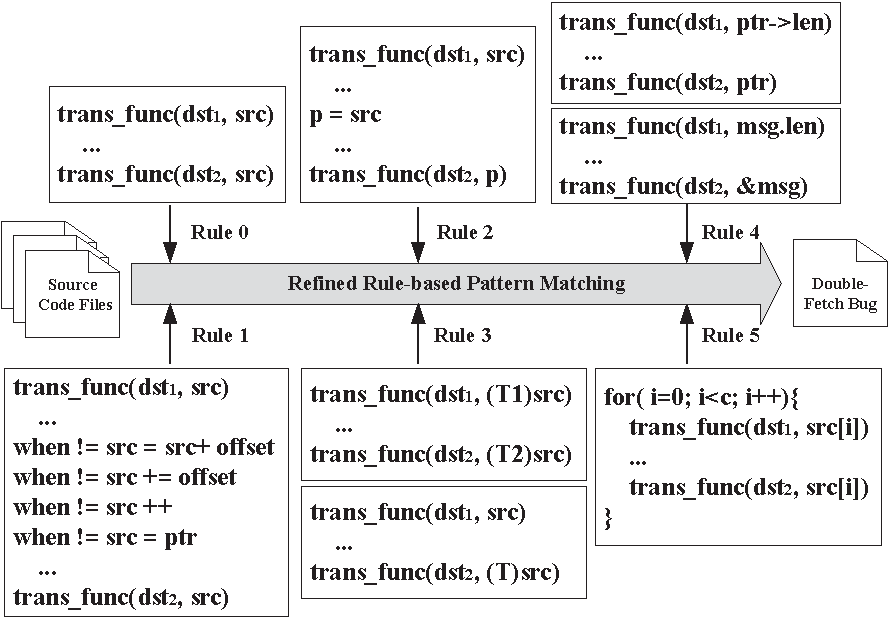
\includegraphics[width=10cm]{refined}
  \caption{Refined Coccinelle-Based Double-fetch Bugs Detection~\cite{wang}}
  \label{Cocci}
\end{figure}


\textbf{Rule 0: Basic pattern matching rule.}
This is the basic scene where two fetches get the data from the exact same user address by invoking the transfer functions. %As to the more complex situations like assignment and pointer, the other five rules are used.

\textbf{Rule 1: No pointer change.}
This rule is used to eliminate the cases when the pointer to the user space changes between two fetches, such as self-increment, adding or subtracting an offset. This rule can reduce the false positive rate of detection.

\textbf{Rule 2: Pointer aliasing.}
There are many pointer changes (assignments) in the kernel code, so different pointers in double fetches can point to the same user address to facilite the data reuse. Wang \textit{et al.} considered one occurrence of pointer assignment between the two fetches to reduce false negatives.
%double fetches to detect this situation as shown in Fig.\ref{Cocci}.

\textbf{Rule 3: Explicit type conversion.}
%不要说些没用的话!下面第一句话的有什么意义?
%Pointer type conversion is always used while fetching data from the user space. At the first fetch, the pointer may be converted to a message header pointer and converted to a whole message pointer at the second fetch. This rule can reduce the false negative rate of detection.
Pointer type conversion is a situation that the pointer is converted to a message header pointer at the first fetch and then, converted to a pointer to the whole message at the second fetch. This rule can reduce the false negative rate of detection.

\textbf{Rule 4: Combination of element fetch and pointer fetch.}
Another complex situation is that the user addresses fetched twice are not exactly the same. For example, at the first fetch, the kernel fetches a data member of a struct such as \verb:ptr->length:, and then, after checking validity or preparation, the kernel fetches the whole struct using \verb:ptr: at the second fetch.

\textbf{Rule 5: Loop involvement.}

The last rule is about loop operations. Since the Coccinelle engine is path-sensitive, 
a loop will be expanded multiple times, i.e., each transfer function will be scanned 
more than one time. Thus, a transfer function at the end of a loop will match with a transfer function at the beginning of the next loop as a double fetch, which should be excluded as the pointer has changed when.





\begin{figure}[t]
  \centering
  %\includegraphics[width=\columnwidth]{f12}
\begin{lstlisting}[style=code]
96   static struct autofs_dev_ioctl * copy_dev_ioctl(struct autofs_dev_ioctl __user *in)
97   {
98    struct autofs_dev_ioctl tmp, *res;
99   
100   if (@copy_from_user(&tmp, in, AUTOFS_DEV_IOCTL_SIZE)@)
101     return ERR_PTR(-EFAULT);
102  
103   if (tmp.size < AUTOFS_DEV_IOCTL_SIZE)
104     return ERR_PTR(-EINVAL);
105  
106   if (tmp.size > AUTOFS_DEV_IOCTL_SIZE + PATH_MAX)
107     return ERR_PTR(-ENAMETOOLONG);
108  
109   res = @memdup_user(in, tmp.size)@;
110   if (!IS_ERR(res))
111     res->size = tmp.size;
	  ...
114  }   
\end{lstlisting}
  \caption{An Undetectable Double-fetch Bug in File \textbf{/fs/autofs4/dev-ioctl.c}}
  \label{dev-ioctl}
\end{figure}




However, these rules are not strong enough to cover all double-fetch bugs, such as function
\verb:copy_dev_ioctl(): in file \verb:/fs/autofs4/dev-ioctl.c:. As Fig.\ref{dev-ioctl} shows, 
in this double-fetch bug, the first fetch occurs at line 100 with a transfer function \verb:copy_from_user(): and the second fetch occurs at line 109 with a function 
\verb:memdup_user():. They both copy the data from the same user address pointed by the 
pointer \verb:in: to the kernel space. However, function \verb:memdup_user: is not one of 
the four transfer functions Wang \textit{et al.} used, so it won't be detected by Wang 
\textit{et al.}'s method. But in fact, function \verb:memdup_user: indeed contains a 
transfer function \verb:copy_from_user(): and some other operations, thus, it can be 
regarded as a transfer function in this case. We improve the rules as follows.


\begin{table}[t!]
\caption{Expanded Transfer Functions}
\centering
\begin{tabular}{ccccc} 
  \hline
  \textbf{No.} & \textbf{Name} & \textbf{Type} & \textbf{Parameter} \\
  \hline
  1 & get\_user & macro & dst, src \\
  2 & \_\_get\_user & macro & dst, src \\
  3 & unsafe\_get\_user & macro & dst, src, err \\
  4 & \_\_copy\_in\_user & macro & des, src, len \\
  5 & \_\_copy\_user & function & dst, src, len \\
  6 & \_\_copy\_user\_zeroing & function & dst, src, len \\
  7 & copy\_from\_user & function & dst, src, len \\
  8 & \_\_copy\_from\_user & macro & dst, src, len \\
  9 & \_\_copy\_from\_user\_inatonmic & macro & dst, src, len \\
  10 & strncpy\_from\_user & function & dst, src, len \\
  11 & strndup\_user & function & src, len \\
  12 & memdup\_user & function & src, len \\
  13 & memdup\_user\_nul & function & src, len \\
  14 & getname\_flags & function & src, flags \\
  15 & getname & function & src \\
  \hline
\end{tabular}
\label{transfer-func}
\end{table}


\textbf{Add more transfer functions.} Wang \textit{et al.} used only four transfer functions in his experiment, \verb:get_user():, \verb:__get_user():, \verb:copy_from_user():, and \verb:__copy_from_user():. However, there are also many other functions containing transfer functions, and their targets are transferring data from user space to kernel space as well, such as \verb:memdup_user(): mentioned above. In addition to funcions, there are also many macros playing the same role in the kernel, like \verb:__copy_from_user_inatomic():.
In the double-fetch bugs detection scenario, these functions and macros can be regarded as transfer functions as well. Table~\ref{transfer-func} shows 15 functions (and macros) we include to detect double-fetch bugs.% detection and their types and parameters. Except for functions used, there are still many functions in kernel meet the condition that transferring data from user space to kernel space, however, many of them have not been used in the code. So these functions are abandoned and lifted efficiency.


\textbf{Fix incomplete rules.}
Rules which Wang \textit{et al.} proposed are theoretically correct. However, in the implementation phase, they were achieved incompletely, which leaded false negatives. For instance, in \verb:/fs/nfsd/nfs4recover.c:, as shown in Fig.\ref{fix}, the first fetch happens at line 730, fetching the data pointed by \verb:&cmsg->cm_xid:, the second fetch happens at line 753, fetching the data pointed by \verb:src:, and there is no assignment or statement between two fetches. According to Rule 2 in section~\ref{design1}, this is not a double-fetch bug. But in fact, this is indeed a double-fetch bug for its assignment happens at line 717. Thus, \verb:cmsg: and \verb:src: point to the same user address actually. This case is missed because of careless implementation. We fixed this kind of rules and reduced the false negative rate.

\begin{figure}[t]
  \centering
  %\includegraphics[width=\columnwidth]{f12}
\begin{lstlisting}[style=code]
714 static ssize_t cld_pipe_downcall(struct file *filp, const char __user  *src, size_t mlen)
715 {
716   struct cld_upcall *tmp, *cup;
717   @struct cld_msg __user *cmsg = (struct cld_msg __user *)src;@
718   uint32_t xid;
719   struct nfsd_net *nn = net_generic(file_inode(filp)->i_sb->s_fs_info, nfsd_net_id);
721   struct cld_net *cn = nn->cld_net;
	  ...
730   if (@copy_from_user(&xid, &cmsg->cm_xid, sizeof(xid)@) != 0) {
731     dprintk("%s: error.", __func__);
732     return -EFAULT;
733   }
	  ...
752 
753   if (@copy_from_user(&cup->cu_msg, src, mlen@) != 0)
754     return -EFAULT;
	  ...
758 }
\end{lstlisting}
  \caption{An Undetectable Double-fetch Bug in File \textbf{/fs/nfsd/nfs4recover.c}.}
  \label{fix}
\end{figure}


\textbf{Remove more non-double-fetch bugs.}
Wang \textit{et al.} used his pattern rules find 90 candidates files in total, it's still a little heavy for technicians to check manually. To lower false positive rate, more situations are added to remove those non-double-fetch bugs:

%\drivers\isdn\i4l\isdn_ppp.c
\textbf{1. The procedure returns after the first fetch.}
As shown in Fig.\ref{return}, there are two fetches at line 850 and 879, and the first fetch is in a \verb:IF: statement. This case will be matched with prior rules apparently. However, there is a \verb:RETURN: statement after the first fetch at line 857, that means, the second fetch will never be executed if the first fetch is executed. Thus, this is not a double-fetch bug actually. There are many cases like this in the kernel code.

\begin{figure}[t]
  \centering
  %\includegraphics[width=\columnwidth]{f12}
\begin{lstlisting}[style=code]
826 int isdn_ppp_write(int min, struct file *file, const char __user *buf, int count)
827 {
	  ...
844     if (lp->isdn_device < 0 || lp->isdn_channel < 0) {
	  ...
850       if (@copy_from_user(protobuf, buf, 4)@)
851         return -EFAULT;
	  ...
857       @return 0;@
858     }
859 
860     if ((dev->drv[lp->isdn_device]->flags & DRV_FLAG_RUNNING) &&
	  ...
878       cpy_buf = skb_put(skb, count);
879       if (@copy_from_user(cpy_buf, buf, count)@)
880       {
881         kfree_skb(skb);
882         return -EFAULT;
883       }
	  ...
904 } 
\end{lstlisting}
  \caption{An Example when Procedure Returns after the First Fetch.}
  \label{return}
\end{figure}

%\drivers\isdn\hysdn\hysdn_procconf.c
\textbf{2. Two fetches are in the different branches.}
Another situation is when the two fetches are in the different branches, just like a \verb:SWITCH: statement. For instance, function \verb:hysdn_conf_write: in \verb:\drivers\isdn\hysdn_procconf.c: is matched with double-fetch bugs detection. But its two fetches are located in the different branches, the first fetch is in the \verb:IF: statement with condition \texttt{cnf->state == CONF\_STATE\_DETECT} and the second fetch is in the \verb:IF: statement with condition \texttt{cnf->state == CONF\_STATE\_POF}. These two conditions can never be satisfied at the same time, so this situation is also a non-double-fetch bug situation.

Besides, based on the improvement mentioned above, we summed up the other two types of double-fetch bugs. They are as follows:

\textbf{1. Validity Checking.}
Validity checking is the situation when the header of a message is fetched to verify the validity of the message. Different from size checking and type selection, this header is only used in the validity verifying, whereas in other cases, the header will be used in memory allocation or \verb:SWITCH: statements.

\textbf{2. Reacquisition.}
Another type is Reacquisition. In this scenario, there is no obvious relation between the two fetches. It simply fetches the data from the same user address twice.


\subsection{Automated Patching with Intel TSX}
\label{design2}

\begin{figure}[htb!]
\begin{algorithmic}[1]
\State \textbf{shared variable:} 
\State ~~~~mutex
\State 
\State \textbf{local variable:} 
\State ~~~~retries
\State
\Procedure{lock}{~}
  \State retries $\gets$ 0
  \State \_xbegin(~) \label{line:xbegin}
  \If {lock\_is\_free(lock)}
  \State \textbf{return}
  \Else 
  \State \_xabort(~)
  \EndIf
  \State retries++
  \If {retries $<$ MAX\_RETRIES}
  \State goto line 9
  \Else
  \State mutex.lock(~) a
  \EndIf
\EndProcedure
\State
\Procedure{unlock}{~}
\If {\_xtest(~)}
\State \_xend(~)
\Else 
\State mutex.unlock(~)
\EndIf
\EndProcedure
\end{algorithmic}
\caption{Speculative lock \& unlock with HTM }
\label{speculative-lock}
\end{figure}




Previous research only proposed suggestions on preventing double-fetch bugs~\cite{wang, precise}, such as don't copy the header twice, use the same value, overwrite the second fetched data, compare data from the two fetches, and synchronize the fetches. However, we need a practical solution to automatically fix the bug.

%\textbf{(1) Don't Copy the Header Twice.} 
%Double-fetch bugs can be thoroughly avoided by changing into one fetch. If there is only one fetch, any malicious change to data will be useless for they won't be fetched into kernel anymore; 
%\textbf{(2) Use the Same Value.} 
%A double-fetch bug can be harmful when the data changed after its validity been checked. This can be solved by using the same value fetched by the first, i.e., ignore the data got by the second fetch; 
%\textbf{(3) Overwrite Data.} 
%Overwriting data which may be changed by the malicious user is also a useful solution. This is always used when the first fetch is a message header, and it overwrites message header after fetching the whole message. This method is widely used in FreeBSD code; 
%\textbf{(4) Compare Data.} 
%Adding a compare operation after the second fetch is another solution. Once the data fetched twice are different, prevention measures will work; 
%\textbf{(5) Synchronize Fetches.} 
%The last method is using synchronized fetches. Traditional synchronization mechanisms used in parallel programs, such as locks, are suitable for resolving double-fetch bugs. They will provide a guarantee of data consistency in the user space. However, this method will sacrifice performance of the system, making itself worthless.

Transactional memory, as an emerging parallel programming paradigm, provides opportunities to facilitate the dynamic schedules via speculative execution. Instead of pessimistically locking the shared memory locations to prevent potential conflicting concurrent updates, transactional executions optimistically elide the lock and speculatively perform memory operations. Thus, transactional memory becomes a promising solution that provides programmer-friendly usability without sacrificing performance.

DFTinker's fixing function is implemented using Intel's Restricted Transactional Memory (RTM) software interface. RTM defines three new instructions: \verb:XBEGIN:, \verb:XEND:, and \verb:XABORT:. Programmers can use \verb:XBEGIN: and \verb:XEND: to specify the begin and end of a hardware transaction and use \verb:XABORT: to explicitly abort a hardware transaction. Additionally, one can adopt the \verb:XTEST: instruction to check whether the processor is executing a code region in transactional execution mode. Due to its best-effort nature, RTM never guarantees successful commit of hardware transactions, which necessitates a fallback path to ensure forward progress.




As Fig.\ref{speculative-lock} shows, a standard mutex lock is employed as the fallback path. 
Our lock method firstly initiates a hardware transaction via \verb:XBEGIN: and checks the state of the mutex immediately at the beginning of the transaction. The locked state of the mutex lock indicates that there is a transaction executing on the fallback path, and all the speculative executions must be canceled. 
If the mutex lock is free, our lock method just returns (without touching the mutex variable) and leaves the processor in the transactional execution mode. Thus, it could perform updates to latents speculatively with zero synchronization overhead. 
Note that this is only a basic fallback scheme in Fig.\ref{speculative-lock} for simplicity, 
more thorough and powerful fallback path could be established through scanning the \textit{abort status} register to get the detailed cause for the abort. 

\begin{table}[t]
  \centering
  \caption{Statistical Results of Detection of Double-fetch Bugs}
  \begin{tabular}{cccccccc}
    \hline
    Kernel & Version & Files & \makecell{Size \\ Checking} & \makecell{Type \\ Selection} & \makecell{Validity \\ Checking} & Reacquisition & \makecell{Total \\ Bugs}\\    
    \hline
    Linux & 4.14.10 & 45614 & 13 & 5 & 4 & 2 & 24 \\
    FreeBSD & 11.1 & 38811 & 7 & 2 & 2 & 1 & 12 \\
    OpenBSD & 6.2 & 29704 & 0 & 0 & 0 & 0 & 0 \\
    Android & 7.0.0 (3.18) & 30479 & 14 & 7 & 5 & 15 & 41 \\
    Darwin & 10.13.3 & 49105 & 3 & 1 & 0 & 0 & 4 \\
    \hline
    \label{stat}
  \end{tabular}
\end{table}




\section{Implementation}%0.5
\label{imple}

%实现是讲你基于什么语言,代码量,什么框架、工具版本等细信息。你下面说的机器信息是实验环境,不一样。
DFTinker is implemented as three SmPL files (2,034 LoC in total) and a shell script file (103 LoC) based on the Coccinelle engine version 1.0.4 with Python support. The three SmPL files are used for detecting double-fetch bugs and filtering out non-double-fetch bugs cases. The Coccinelle engine will use these files as pattern rules to find double-fetch bugs. The shell script is used for supervising the Coccinelle engine and sorting out the results of the experiments.


\section{Evaluation}%1.5
\label{evalue}
This section will discuss DFTinker's ability to detect double-fetch bugs and the performance of the operating system fixed by DFTinker.


\subsection{Detection of Double-fetch Bugs}
\label{evalue1}
The experiment was conducted on a Linux laptop running Ubuntu 16.04 x64, with one Intel i7-7700HQ 2.6GHz processor, 8GB of memory, 250GB SSD. We used Linux 4.14.10, OpenBSD 6.2, FreeBSD 11.1, Android 7.0.0 (kernel version 3.18), and Darwin 10.13.3, which were the relatively newer version when the experiment was conducted. To prove that DFTinker can find out bugs reported by prior works, the experiment was also conducted on Linux 4.5, the same version Wang \textit{et al.} used to experiment on.


At first, DFTinker was run with the Linux kernel 4.5, so as to confirm Wang \textit{et al.}'s work. DFTinker successfully reached Wang \textit{et al.}'s result. All five known double-fetch bugs (CVE-2016-5728, CVE-2016-6130, CVE-2016-6136, CVE-2016-6156, CVE-2016-6480)
reported in Linux kernel 4.5 were found, which proved that DFTinker has the same effectiveness as Wang
\textit{et al.}'s work in detecting double-fetch bugs.


Then, DFTinker was applied to the five prevalent open source kernels. The statistical result is shown in Table~\ref{stat} and parts
\footnote{Due to the space limitation of the page, the full results of the double-fetch bugs are available at https://github.com/luoyyqq}​ of the detailed results are shown in Table~\ref{result}.

\textbf{1. Linux.} The Linux kernel used is version 4.14.10 which was released on Dec 29, 2017. In this version, five double-fetch bugs reported by Wang \textit{et al.} had already been fixed, but DFTinker still found 24 cases in total.

\begin{table*}[htb!]
  \centering
  \caption{Part of the Detailed Results of Double-fetch Bugs}
  \begin{tabular}{cccccc}
    \hline
    No. & File & Function & \makecell{Line of the\\First Fetch} & \makecell{Line of the\\Second Fetch}  & Type  \\  
    \hline
    1 & bus.c & \_\_nd\_ioctl & 942 & 1025 & Type-selection \\
2 & commctrl.c & ioctl\_send\_fib & 82 & 119 & Size-checking \\
3 & megaraid\_mm.c & mega\_m\_to\_n & 3443 & 3467 & Validity-checking \\
	...\\ 
	\hline
25 & aac.c  & aac\_ioctl\_sendfib() & 2999 & 3007 & Size-checking \\
26 & aacraid.c  & aac\_ioctl\_sendfib() & 2763 & 2771 & Size-checking \\
27 & bcm2835\_vcio.c  & vcio\_ioctl() & 66 & 72 & Size-checking \\
...\\
\hline
37 & signal\_32.c & do\_sigreturn & 86 & 93 & Validity-checking \\
38 & tcp.c & do\_tcp\_getsockopt & 2774 & 2823 & Reacquisition \\
39 & ft1000\_debug.c & ft1000\_ioctl & 551 & 566 & Size-checking \\
...\\
	\hline
78 & dtrace.c & dtrace\_dof\_copyin & 11602 & 11626 & Size-checking \\
79 & nfs\_syscalls.c & fhopen & 620 & 626 & Size-checking \\
80 & nfs\_vfsops.c & nfs\_vfs\_mount & 1834 & 1872 & Type-selection \\
81 & ucode.c & copyin\_update & 92 & 117 & Size-checking \\
\hline
    \label{result}
  \end{tabular}
\end{table*}

\textbf{2. FreeBSD.}
%有几个人不认识FreeBSD?需要费工夫介绍么?下同
%FreeBSD is an open-source Unix-like operating system, which is the most widely used open-source BSD distribution. 
The FreeBSD version was 11.1, which was released in July 2017. Note that FreeBSD is a little different from Linux, for FreeBSD uses \verb:copyin(): and \verb:copyin_nofault(): as transfer functions. Thus, it needs to modify corresponding pattern code in DFTinker before the experiment. In FreeBSD, 12 cases were found in total.



\textbf{3. OpenBSD.}
%OpenBSD is also an open-source UNIX-like operating system and it is one of the three popular distributions of BSD. 
The OpenBSD version tested is 6.2, which was released in Oct 2017. In our experiment, DFTinker didn't find any double-fetch bug in OpenBSD. In fact, OpenBSD provides many security features in the system which are optional or unavailable in other operating systems, and developers audit source code for security frequently. This may be the reason why DFTinker can't find any double-fetch bug in OpenBSD.

\textbf{4. Android.}
Android is a special distribution of Linux. It uses Linux kernel with specific modification. The Android version tested was 7.0.0 based on Linux kernel version 3.18. We found 41 double-fetch bugs in the Android kernel source.

\textbf{5. Darwin.}
Darwin is a Unix operating system which was open-sourced by Apple Inc. in 2000. In our experiments, we chose Darwin version 10.13.3, which was the latest version when we conducted the experiments. Similar to FreeBSD, Darwin uses \verb:copyin(): and \verb:copyin_nofault(): as transfer functions, so we can directly use FreeBSD version DFTinker. We totally found 4 double-fetch bugs in Darwin.

\subsection{Automated Patching with Intel TSX}
\label{evalue2}




To evaluate the efficiency of the fixed operating system, another Ubuntu 14.04 x64 was implemented. We chose five vulnerable functions from the detection results and fixed them by DFTinker. By comparing the run time of the invocation of the vulnerable functions before fixing and after fixing, we could get the performance overhead of DFTinker. This operating system ran on a server with a 4-core Intel Core i7-6700 CPU (clocked at 3.40GHz, supporting RTM) with each core possessing a private 32KB L1 cache and a private 256KB L2 cache and a shared 8MB L3 cache. The memory was 32GB and the storage was a 250GB SSD.


As Coccinelle engine is accurate in locating lines of double-fetch bugs in the code, it is easy to fix \verb:LOCK(): and \verb:UNLOCK(): operations to the code. According to the feature of transaction memory, all operations between \verb:LOCK(): and \verb:UNLOCK(): will be executed in a transaction, execution results will be committed if there are no conflicts. In other words, if there is a malicious user changes the data in the user space after the first fetch, all operations in the transaction will be aborted and rerun from \verb:LOCK():, which guarantees the consistency of the data. In our experiments, we fixed target functions using DFTinker and modified the data between two fetches using a user thread. The results showed that the data fetched at the second time was same as the first time, which proved that DFTinker was effective in protecting double-fetch bugs.

To evaluate the overhead performance of the fixed code, an Ubuntu 14.04 x64 was used, whose kernel version was 4.6.1. DFTinker was used to fix the functions in the Table~\ref{performance}. Then, a program ran to call the target function for a thousand times and recorded its runtime. At last, it was compared with the runtimes that ran on the operating system not been fixed. After testing for twenty times and taking the average, the fixed operating system owned a decent overhead performance of 1.3~\%. The detailed results were shown in Table~\ref{performance}.


\begin{table}[t!]
\caption{Results of the Performance Tests of the Fixed Code}
\centering
\begin{tabular}{ccccc} 
  \hline
Vulnerable Functions & Files & \makecell{Origin \\ Runtime (\textmu s)} & \makecell{Fixed \\ Runtime (\textmu s)} & \makecell{Average \\ Overhead} \\
\hline
ioctl\_file\_dedupe\_range() & ioctl.c & 556.25 & 563.25 & 1.3\% \\
ll\_dir\_ioctl() & dir.c & 438.72 & 444.12 & 1.2\% \\
copy\_dev\_ioctl() & dev-ioctl.c & 659.43 & 668.86 & 1.4\% \\
\_ctl\_ioctl\_main() & mpt3sas\_ctl.c & 445.12 & 450.11 & 1.1\% \\
sg\_scsi\_ioctl() & scsi\_ioctl.c & 515.12 & 522.02 & 1.3\% \\

  \hline
\end{tabular}
\label{performance}
\end{table}

\section{Discussion}%1
\label{discuss}

Double-fetch bugs are significant problems in the operating systems, and they have been found in almost all the modern kernels, such as the Windows, Linux, FreeBSD, and Android~\cite{wang,precise}. Double-fetch bugs have a long history, and some of them existed over 10 years (CVE-2016-6480). Besides, potential double-fetch bugs (currently not buggy) can turn into buggy ones when the code is updated without paying special attention to the double fetch issue, such as CVE-2016-5728 and CVE-2016-6516. Wang \textit{et al.}~\cite{wang} call such situations as benign double-fetch situations and paid special attention to them. Xu \textit{et al.}\cite{precise} regarded such potential bugs as real bugs. Thus, in this paper, we take all the potential double-fetch bug situations into consideration as well to conduct a thorough detection and fix.

We have implemented a tool named DFTinker to automatically detect and fix double-fetch bugs. DFTinker can analyze the whole kernel (including all drivers) in one execution, which has a good code coverage. In addition, DFTinker can detect and fix the bug at the same time, which is efficient. Furthermore, it can prevent the potential double-fetch bug that is undetectable with current approaches, such as the special double-fetch bug (CVE-2015-8550) introduced by the compiler~\cite{wilhelm15tracing}.

Although DFTinker achieves a decent performance in detecting and fixing double-fetch bugs, it relies on the availability of the source code, which is suitable for in-house testing. We will take the binary situations into consideration in the future work. 

%It cannot handle the special case that the double-fetch bug does not reside in the source code but is introduced by the compiler (CVE-2015-8550)~\cite{wilhelm15tracing}. We will include such situations in the future work. 


%\begin{itemize}
%\item DFTinker cannot find out double-fetch bugs with unknown transfer functions. In fact, there are many other functions contains one or more transfer functions, so these functions can be regarded as transfer functions, too. However, it is not easy for a static method to identify whether a function call transfer functions finally or not. This is left for future work.
%\item DFTinker cannot figure out double-fetch bugs introduced by compilers, like CVE-2015-8550~\cite{wilhelm15tracing}. As DFTinker works on source code level, any double-fetch bug happens in lower level cannot be found. It may be detected by a dynamic approach. Nevertheless, DFTinker can prevent such bugs with our prevention approach based on transactional memory.
%\end{itemize}



%我说过两次让你把related work单独做一节,不要放在discussion里!
\section{Related Work}
\label{related}

%Both double-fetch bugs and transactional memory are widely studied nowadays.

%\textbf{Double-fetch bugs.} Similar to program analysis, methods used to study double-fetch bugs can be divided into dynamic and static.

Jurczyk and Coldwind~\cite{bochspwn,jurczyk2013identifying} used a dynamic approach in their Bochspwn project to study double-fetch bugs in Windows. By tracing memory accesses, they successfully found double-fetch bugs in the Windows kernel. Wilhelm~\cite{wilhelm15tracing} used an approach similar to the
Bochspwn project to analyze memory access pattern of para-virtualized
devices' backend components. His analysis discovered three novel security
vulnerabilities in security-critical backend components. One of the
discovered vulnerabilities does not exist in the source code but is
introduced through compiler optimization.
Inherently, such dynamic approaches have a low code coverage, i.e., code under strict conditions may never be tested. Furthermore, code that is being tested is limited to the emulation ability, causing double-fetch bugs in hardware devices that it cannot emulate may be missed. Our static approach has a better code coverage and can detect double-fetch bugs in the drivers, where the dynamic approaches are incapable of.

%Prior works have already studied double-fetch bugs in Windows~\cite{hammou2016exploiting,jurczyk2013identifying,bochspwn} and Linux~\cite{wang,Wang2017A,precise,modern} systems. Bochspwn~\cite{bochspwn,hammou2016exploiting} used a dynamic approach to detect double-fetch bugs on Windows. Bochspwn defines a short time frame. Once an access to a user address happened twice in the time frame, it will be sorted as a double-fetch bug. Obviously, Bochspwn owns a low code coverage for code that under strict conditions may be never tested. Furthermore, code that Bochspwn can test is limited to its emulation ability, causing double-fetch bugs in hardware devices that it cannot emulate may be missed.

Wang \textit{et al.}~\cite{wang} is the first to systematically study double-fetch bugs in the Linux kernel. Based on the transfer functions, they use a static pattern-matching approach to detect double-fetch bugs. In addition to the identification of six real double-fetch bugs, they also propose five solutions to prevent double-fetch bugs. However, the accuracy of their detection approach is undesirable and they could not automatically fix the bug after identifying them. % And because of the incomplete model of the double-fetch bug, its accuracy is undesirable and the false alarm rate is quite high.
Our approach can automatically detect and fix double-fetch bugs at the same time.

%相关工作是简述别人工作后着重说人家不足,你把人家工作写的那么认真那么好,你还做什么?
Schwarz \textit{et al.}~\cite{modern} proposed a method using cache-attack and kernel-fuzzing techniques to detect, exploit, and eliminate double-fetch bugs in Linux syscalls. %These techniques were efficacious according to the experiment results that the exploitation success rate reached up to 97\%. Schwarz \textit{et al.} also used hardware transactional memory to eliminate double-fetch bugs. They achieved a mechanism named DropIt with a performance overhead of 0.8\%. 
However, their approach is limited to Linux syscalls, whereas large numbers of the double-fetch bugs occur in non-syscall functions, such as functions in drivers, are missed. Thus, their approach suffers from a low code coverage, whereas our approach is free from that.% for its inherent characteristics.

Xu \textit{et al.}\cite{precise} proposed a formal definition of double-fetch bugs and used a static analysis based on LLVM IR and symbolic execution to detect such bugs. However, their definition takes all the potential situations into consideration, which are not currently buggy but only have the potential to turn into bugs when the code is updated. Besides, their approach needs to compile the source code to LLVM IR and specify the target architecture. Thus, it detects only one architecture at one time, leading to the miss of bugs such as CVE-2016-6130. Our approach has a better code coverage, which can analyze the source code of all the architecture at one time. We also provide automatical fix after the bug is identified, which is efficient than previous works.

%人家的符号执行不是传统的执行,不需要fork分支去执行,所以没有空间爆炸问题。
%also studied double-fetch bugs in the Linux kernel. They proposed a formal definition of double-fetch bugs and implemented a static analysis system named DEADLINE. Their approach needed to compile the source code to LLVM IR, and checking authenticity with a modified symbolic execution method. However, when the source code was compiled to LLVM IR, it needed to specify the target architecture, thus, the system would detect only one architecture at once, leading to the miss of CVE-2016-6130. And it had common failings of the symbolic execution, such as the path explosion and constraint solving difficulties.



%In our approach, we used a source-level static analysis method, which could cover all architectures in one process and owned a high code coverage. Besides, our better model led to a higher accuracy and lower false alarm rate.


%你研究的是double fetch,不是TM,相关工作需要double fetch的工作,不需要TM!
%\textbf{Transactional memory.} Transactional memory~\cite{Herlihy1993Transactional,Hammond2004Transactional,Harris2010Transactional}, as an emerging programming paradigm, has attracted great attention. With transactional memory, programmers can easily implement fine-grained operations.

%Most of the time, transactional memory is used as a substitute for the lock mechanism in parallel programming~\cite{Herlihy1993Transactional}, but recently, it has been applied to other fields as well.

%Guan \textit{et al.}~\cite{Guan2015Protecting} used hardware transactional memory to protect private keys in memory, it could deal with information disclosure attacks efficaciously. Jang \textit{et al.}~\cite{Jang2016Breaking} used hardware transactional memory to break kernel address space layout randomization, which is the core mechanism of the preventing systems from memory attacks, such as buffer overflow.

%The transactional memory is successfully applied to the double-fetch bugs protection as well. With its feature, DFTinker can guarantee the consistency of data between two fetches, which can solve double-fetch bugs radically.



\section{Conclusion}
\label{conclusion}

This paper proposes an approach to automatically detect and fix double-fetch bugs. We implement a prototype named DFTinker and evaluate it with real kernels. Experiments show that DFTinker is effective and efficient in automatically detecting and fixing double-fetch bugs. DFTinker detected 81 cases in prevalent kernels and the performance overhead of the fixed program is only 1.3\% on average.

%, we implemented a prototype named DFTinker, which could detect double-fetch bugs and fix code automatically. With more transfer functions, DFTinker identified more double-fetch bug situations and owned a higher accuracy. With stricter rules, DFTinker filtered double-fetch bugs where it couldn't result in fatal errors, lowering false alarm rate significantly. In total, DFTinker detected 24 cases in Linux 4.14.10, 12 cases in FreeBSD 11.1, and no case in OpenBSD 6.2 and Android 7.0.0. Finally, DFTinker used hardware transactional memory to prevent double-fetch bugs, which is efficacious and with a performance overhead of only 1.3\%.

% \section*{Acknowledgment}


% The authors would like to thank...

% \ifCLASSOPTIONcaptionsoff
%   \newpage
% \fi

\bibliography{journal}
\bibliographystyle{abbrv}

\end{document}



% \begin{table*}[htb!]
%   \centering
%   \caption{Results of Double-fetch Bugs Detection}
%   \begin{tabular}{cccccc}
%     \hline
%     No. & File & Function & the First Fetch & the Second Fetch & Type  \\   
%     \hline
%     1 & bus.c & \_\_nd\_ioctl & 942 & 1025 & Type-selection \\
% 2 & commctrl.c & ioctl\_send\_fib & 82 & 119 & Size-checking \\
% 3 & compat.c & cmsghdr\_from\_user\_compat\_to\_kern & 138 & 167 & Size-checking \\
% 4 & core.c & sched\_copy\_attr & 4342 & 4381 & Size-checking \\
% 5 & core.c & perf\_copy\_attr & 9639 & 9676 & Size-checking \\
% 6 & custom\_method.c & cm\_write & 37 & 54 & Size-checking \\
% 7 & dev-ioctl.c & copy\_dev\_ioctl & 100 & 109 & Size-checking \\
% 8 & dir.c & ll\_dir\_ioctl & 1485 & 1504 & Size-checking \\
% 9 & dpt\_i2o.c & adpt\_i2o\_passthru & 1734 & 1834 & Type-selection \\
% 10 & hpioctl.c & asihpi\_hpi\_ioctl & 131 & 140 & Size-checking \\
% 11 & ioctl.c & ioctl\_file\_dedupe\_range & 586 & 597 & Size-checking \\
% 12 & llite\_lib.c & ll\_copy\_user\_md & 2463 & 2478 & Size-checking \\
% 13 & megaraid\_mm.c & mega\_m\_to\_n & 3443 & 3467 & Validity-checking \\
% 14 & mpt3sas\_ctl.c & \_ctl\_ioctl\_main & 2261 & 2311 & Validity-checking \\
% 15 & nfs4recover.c & cld\_pipe\_downcall & 730 & 753 & Validity-checking \\
% 16 & opal-prd.c & opal\_prd\_write & 238 & 244 & Size-checking \\
% 17 & psdev.c & coda\_psdev\_write & 109 & 128 & Type-selection \\
% 18 & scsi\_ioctl.c & sg\_scsi\_ioctl & 440 & 466 & Size-checking \\
% 19 & tls\_main.c & do\_tls\_setsockopt\_tx & 351 & 379 & Type-selection \\
% 20 & uhid.c & uhid\_event\_from\_user & 407 & 455 & Type-selection \\
% 21 & util.c & strndup\_user & 187 & 195 & Size-checking \\
% 22 & vhost.c & vhost\_vring\_ioctl & 1361 & 1379 & Validity-checking \\
% 23 & vt.c & con\_font\_set & 4135 & 4152 & Reacquisition \\
% 24 & wext-core.c & ioctl\_standard\_iw\_point & 747 & 809 & Reacquisition \\
%   \hline
% 25 & aac.c  & aac\_ioctl\_sendfib() & 2999 & 3007 & Size-checking \\
% 26 & aacraid.c  & aac\_ioctl\_sendfib() & 2763 & 2771 & Size-checking \\
% 27 & bcm2835\_vcio.c  & vcio\_ioctl() & 66 & 72 & Size-checking \\
% 28 & dtrace.c  & dtrace\_dof\_copyin() & 13210 & 13234 & Size-checking \\
% 29 & fasttrap.c  & fasttrap\_ioctl() & 2277 & 2294 & Size-checking \\
% 30 & freebsd32\_misc.c  & freebsd32\_jail() & 2300 & 2311 & Type-selection \\
% 31 & hwpmc\_x86.c  & pmc\_save\_user\_callchain() & 112 & 128 & Reacquisition \\
% 32 & kern\_jail.c  & sys\_jail() & 263 & 274 & Type-selection \\
% 33 & linux\_futex.c  & linux\_sys\_futex() & 816 & 819 & Validity-checking \\
% 34 & netmap\_pt.c  & ptnetmap\_read\_cfg() & 779 & 790 & Size-checking \\
% 35 & oce\_if.c  & oce\_handle\_passthrough() & 2293 & 2305 & Size-checking \\
% 36 & sys\_capability.c  & sys\_cap\_rights\_limit() & 259 & 267 & Validity-checking \\
%   \hline
% 37 & af\_decnet.c & \_\_dn\_getsockopt & 1525 & 1582 & Reacquisition \\
% 38 & mpt2sas\_ctl.c & \_ctl\_ioctl\_main & 2158 & 2196 & Validity-checking \\
% 39 & dpt\_i2o.c & adpt\_i2o\_passthru & 1750 & 1855 & Reacquisition \\
% 40 & hpioctl.c & asihpi\_hpi\_ioctl & 132 & 141 & Size-checking \\
% 41 & core.c & atomic\_operation & 136 & 145 & Validity-checking \\
% 42 & auditsc.c & audit\_log\_single\_execve\_arg & 1032 & 1052 & Size-checking \\
% 43 & af\_ax25.c & ax25\_setsockopt & 551 & 646 & Reacquisition \\
% 44 & custom\_method.c & cm\_write & 37 & 54 & Size-checking \\
% 45 & psdev.c & coda\_psdev\_write & 109 & 128 & Type-selection \\
% 46 & dm-ioctl.c & copy\_params & 1619 & 1661 & Reacquisition \\
% 47 & cxgb3\_main.c & cxgb\_extension\_ioctl & 2134 & 2147 & Type-selection \\
% 48 & dhd\_linux.c & dhd\_ethtool & 3542 & 3548 & Type-selection \\
% 49 & traps.c & do\_cpu & 1068 & 1070 & Reacquisition \\
% 50 & ip\_sockglue.c & do\_ip\_setsockopt & 483 & 682 & Reacquisition \\
% 51 & ipv6\_sockglue.c & do\_ipv6\_setsockopt & 136 & 431 & Reacquisition \\
% 52 & keyboard.c & do\_kdgkb\_ioctl & 437 & 445 & Size-checking \\
% 53 & signal\_32.c & do\_sigreturn & 86 & 93 & Validity-checking \\
% 54 & tcp.c & do\_tcp\_getsockopt & 2774 & 2823 & Reacquisition \\
% 55 & ft1000\_debug.c & ft1000\_ioctl & 551 & 566 & Size-checking \\
% 56 & fhandle.c & handle\_to\_path & 182 & 200 & Size-checking \\
% 57 & sys\_hpux.c & hpux\_sysfs & 442 & 452 & Size-checking \\
% 58 & i2o\_config.c & i2o\_cfg\_passthru & 826 & 936 & Reacquisition \\
% 59 & commctrl.c & ioctl\_send\_fib & 81 & 116 & Size-checking \\
% 60 & wext-core.c & ioctl\_standard\_iw\_point & 714 & 776 & Reacquisition \\
% 61 & isdn\_ppp.c & isdn\_ppp\_write & 820 & 846 & Type-selection \\
% 62 & megaraid.c & mega\_m\_to\_n & 3466 & 3490 & Validity-checking \\
% 63 & swarm\_cs4297a.c & mixer\_ioctl & 1465 & 1470 & Size-checking \\
% 64 & af\_netlink.c & netlink\_setsockopt & 1911 & 1971 & Reacquisition \\
% 65 & core.c & perf\_copy\_attr & 6367 & 6404 & Size-checking \\
% 66 & rtl871x\_ioctl\_linux.c & r8711\_wx\_read32 & 1869 & 1874 & Reacquisition \\
% 67 & sg.c & sg\_read & 396 & 409 & Reacquisition \\
% 68 & scsi\_ioctl.c & sg\_scsi\_ioctl & 450 & 470 & Size-checking \\
% 69 & control\_compat.c & snd\_ctl\_elem\_add\_compat & 353 & 356 & Reacquisition \\
% 70 & sock.c & sock\_setsockopt & 640 & 757 & Reacquisition \\
% 71 & 3w-xxxx.c & tw\_chrdev\_ioctl & 911 & 933 & Size-checking \\
% 72 & 3w-9xxx.c & twa\_chrdev\_ioctl & 671 & 693 & Size-checking \\
% 73 & 3w-sas.c & twl\_chrdev\_ioctl & 776 & 798 & Size-checking \\
% 74 & uhid.c & uhid\_event\_from\_user & 279 & 327 & Type-selection \\
% 75 & vhost.c & vhost\_vring\_ioctl & 620 & 638 & Validity-checking \\
% 76 & wl\_priv.c & wvlan\_uil\_put\_info & 606 & 639 & Type-selection \\
% 77 & yam.c & yam\_ioctl & 956 & 979 & Type-selection \\
%   \hline
% 78 & ucode.c & copyin\_update & 92 & 117 & Size-checking \\
% 79 & dtrace.c & dtrace\_dof\_copyin & 11602 & 11626 & Size-checking \\
% 80 & nfs\_vfsops.c & nfs\_vfs\_mount & 1834 & 1872 & Type-selection \\
% 81 & nfs\_syscalls.c & fhopen & 620 & 626 & Size-checking \\
%   \hline

%     \label{result}
%   \end{tabular}
% \end{table*}